\chapter{O \textit{FS-Join}}
\label{cap:cap2}

Este capítulo é destinado à apresentação do framework proposto no trabalho de Rong et al. (2017)\cite{Rong:2017:FS-Join}. Aqui é exposto a arquitetura do \textit{FS-Join} proposta por Rong et al. (2017) \cite{Rong:2017:FS-Join}, com as devidas adequações às tecnologias utilizadas neste trabalho, são discutidos o particionamento vertical, os filtros propostos por Rong et al. (2017)\cite{Rong:2017:FS-Join}, e será apresentado o algoritmo do \textit{FS-Join} tal como foi implementado. Neste trabalho não foi considerado o que Rong et al. (2017)\cite{Rong:2017:FS-Join} chama de particionamento horizontal.

\section{A arquitetura do \textit{FS-Join}}

A arquitetura do \textit{FS-Join} proposta por  Rong et al. (2017) \cite{Rong:2017:FS-Join} pode ser particionada em três etapas: Ordenação, Filtragem e Verificação. Cada um dessas etapas serão exploradas à seguir, ressaltando que, este trabalho preservou a arquitetura original e serão descritas como são realizadas as operações utilizando o \textit{Spark}, enquanto no trabalho original utiliza-se o \textit{MapReduce}, como destacado no capítulo anterior.

\subsection{Ordenação}

Nesta etapa será ordenada toda coleção de caracteres recebidos como entrada. Então, o primeiro passo a ser executado no \textit{FS-Join} é realizar uma ordenação global dos dados recebidos, essa ordenação sera representada por $O$. O método de ordenação utilizado por \cite{Rong:2017:FS-Join} é dividido em duas fases, sendo elas:
\begin{enumerate}
\item  Calcular a frequência para cada \textit{token};
\item  Classificar os \textit{tokens} em ordem crescente tomando como parâmetro de ordenação a frequência do \textit{token}.
\end{enumerate}

O algoritmo que calcula a frequência para a ordenação global do\textit{ FS-Join} utiliza funções do \textit{Spark} para calcular a frequência e obter a ordem global da coleção de \textit{strings} que estão em um \textit{RDD} recebidos como entrada.

\subsection{Filtragem}

Nesta etapa o \textit{FS-Join} utiliza uma função do \textit{Spark} para gerar pares de \textit{strings} candidatos removendo os pares dissimilares sem calcular necessariamente calcular os valores precisos de similaridade.  Segundo \cite{Rong:2017:FS-Join} esta é a operação principal do \textit{FS-Join} é composta por duas fases, que serão descritas à seguir, sendo elas: fase de particionamento e fase de junção. 

Na fase de particionamento, é recebido como entrada o \textit{RDD} contendo as \textit{strings} originais e os \textit{tokens} em ordenação global $O$, obtidas na etapa anterior, e seleciona um número de \textit{pivôs} a partir de $O$ (mais detalhes nas próximas seções). Em seguida, ordena os {tokens} nas \textit{strings} recebidas de acordo com a a ordem global $O$ e particiona cada uma das \textit{strings} em vários \textit{segmentos} utilizando cada um dos \textit{pivôs} que foram cuidadosamente selecionados.  os \textit{tokens} em cada sequência recebida de acordo com a ordem global, cada sequência em vários segmentos com base em um conjunto de \textit{pivôs} cuidadosamente escolhidos (mais detalhes nas próximas seções). 

Após todas essas fases, o \textit{FS-Join} irá tratar o \textit{ID}\footnote{ID - Identificador do objeto gerado, que pode ser um número ou um \textit{token}} da partição como chave,  e o valor correspondente como valor, ao enviar para função \textit{Map}.  Os segmentos pertencentes à mesma partição serão ordenados no mesmo nó de redução. Em cada redutor, o \textit{gerador de chaves candidatas} do \textit{FS-Join} gera candidatos usando um índice invertido baseado em prefixo e vários métodos de filtragem, por exemplo, filtragem por comprimento, filtragem com reconhecimento de \textit{segmento} (veja a próxima seção). A saída do $i$-ésimo redutor é uma lista de pares $(p, c)$, onde $p = (s, t)$ é um par de strings, enquanto $c$ é o número de \textit{tokens} comuns entre $s$ e $t$ na $i$-ésima partição, ou seja, o $i$-ésimo segmento de $s$ e $t$.

\subsection{Verificação}

Durante a etapa de verificação, que é a ultima etapa executada pelo \textit{FS-Join} irá utilizar uma função do \textit{Spark}  para verificar os \textit{candidatos} gerados na fase de filtro anterior. Se o número final de \textit{tokens} comuns de um par de strings for maior que um \textit{threshold}\footnote{\textit{Threshold} - valor limite} $\sigma$, então é uma resposta aceita. Caso contrário, não é. Os detalhes serão discutidos nas próximas seções.
\begin{figure}[ht]
\centering
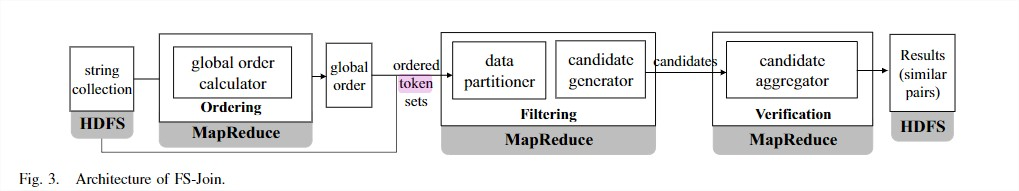
\includegraphics[scale=0.4]{fig/arqFSJoin.jpg}
\caption{Arquitetura do \textit{FS-Join}}
\end{figure}

\section{Particionamento Vertical}



\section{O Algoritmo do \textit{FS-Join}}

%\input{./tabelas/similarCalc}
\begin{algorithm2e}[H]
\DontPrintSemicolon % Some LaTeX compilers require you to use \dontprintsemicolon instead
\Entrada{Uma coleção de conjuntos C; um \emph{threshold} $\theta$}
\Saida{Um conjunto D que contêm todos os pares $(x_1, x_2)$, em que $sim(x_1, x_2) \ge \gamma$}
$I_1, I_2, \dots I_u \gets \emptyset$ \;
$D \gets \emptyset$ \; 
\For{$x_1 \in C$ }{
  $M \gets $ um mapa vazio do conjunto, id e ps (ps = pontuação de sobreposição)\;
  $M(id, ps) \gets \emptyset$ \;
  \For{$t \in$ maxprefix$(x_1)$}{ \;
    Remove todos $x_2 \in I_t$, em que $|x_2| < $ minsize$(x_1)$ \;
    \For{$x_2 \in I_t$}{ \;
        M$(x_2) \gets$ (M$(x_2)$.ps + 1) \;
        \If{}{ \;
        }
    }
  }

  $i \gets i + 1$\; 
}
\Return{location};
\caption{Algoritmo FS-Join}
\label{algo:duplicate}
\end{algorithm2e}

